\begin{center}
	\section{Marco te\'orico}
\end{center}

\noindent
\justify

El marco te\'orico se compone de los siguientes temas: 

\begin{itemize}
	\item M\'etodo de dispersi\'on de la matriz en fase s\'olida: m\'etodo ampliamente usado a escala de laboratorio para la extracci\'on de analitos de inter\'es de extractos procedentes de muestras biol\'ogicas. La planta de extracci\'on desarrollada fue dise\~nada con base en este m\'etodo experimental.
	\item Din\'amica de Fluidos Computacional: herramienta computacional ampliamente usada para el an\'alisis de procesos que emplean fluidos de car\'acter laminar o turbulento, gaseoso o l\'iquido y de tipo Newtoniano o no Newtoniano.
	\item M\'etodo de Elementos Discretos: m\'etodo num\'erico que permite modelar la interacci\'on din\'amica de procesos mec\'anicos que emplean part\'iculas. 
	\item M\'etodo CFD-DEM: acoplamiento entre la Din\'amica de Fluidos Computacional (CFD, por sus siglas en ingl\'es) y el M\'etodo de Elementos Discretos (DEM, por sus siglas en ingl\'es). Permite analizar problemas que emplean tanto fluidos como part\'iculas.
	\item Sedimentaci\'on: expone el fen\'omeno f\'isico base empleado para la separaci\'on de mezclas s\'olido-l\'iquido. A su vez, explica los sistemas de sedimentaci\'on conocidos en la literatura; enfoc\'andose en la metodolog\'ia de dise\~no te\'orico de sedimentadores de placas inclinadas para la propuesta de un dise\~no inicial del sistema de eluci\'on y filtrado de la planta de extracci\'on.
\end{itemize}

\subsection{M\'etodo de Dispersi\'on de la Matriz en Fase S\'olida}	\label{MSPD_chap}

\noindent
\justify

El m\'etodo de dispersi\'on de la matriz en fase s\'olida (MSPD, por sus siglas en ingl\'es) ha sido ampliamente utilizado para el estudio de muestras biol\'ogicas$^{\cite{barker2007, Capriotti2015, Perez2019}}$. Existen m\'as de 250 publicaciones en las que se emplea este m\'etodo extractivo para el an\'alisis de extractos de distintas naturalezas $^{\cite{barker2007}}$. Esto se debe a la alta eficiencia y bajo costo de este m\'etodo de extracci\'on. 

\noindent
\justify

Consiste, b\'asicamente, de tres etapas (como se puede observar en la Figura \ref{mspd}):

\begin{enumerate}
	\item Maceraci\'on de la muestra con un \textit{agente dispersante} (material particulado, normalmente compuesto de s\'ilice).
	\item Homogenizaci\'on de la muestra macerada en la columna.
	\item Eluci\'on con solvente y filtrado de la mezcla \textit{solvente - extracto}.
\end{enumerate}

\begin{figure}[h!]
\centering
\includegraphics[width=0.8\textwidth]{Images/mspd.PNG}
\caption{M\'etodo MSPD$^{\cite{Capriotti2015}}$.}
\label{mspd}
\end{figure}

\subsubsection{Factores a considerar en la extracci\'on MSPD}

\noindent
\justify

Hay varios factores a considerar en la extracci\'on MSPD, que incluye:

\begin{enumerate}
	\item \textit{Efecto del tama\~no de part\'icula media:} tama\~nos de part\'icula peque\~nos (entre $3$ - $10 \, \mu m ^{\cite{barker2007}}$) requiere de grandes tiempos de eluci\'on y altos gradientes de presi\'on para obtener un flujo adecuado. 
	\item \textit{Agente dispersante:} el uso de silicatos infravalorados, como la arena de r\'io, para la maceraci\'on de muestras presenta resultados diferentes a los reportados con agentes dispersantes como el $C_{18}$ o el $C_8$. A pesar de que el mismo principio de disrupci\'on de la matriz se conserva, debido a la abrasi\'on, es probable que se de una interacci\'on qu\'imica no deseada entre silicatos infravalorados y algunos de los flavonoides del extracto.
	\item \textit{Relaci\'on m\'asica:} la mejor relaci\'on m\'asica reportada en la literatura frecuenta ser una relaci\'on 1 a 4 $^{\cite{barker2007}}$, aunque puede variar de una aplicaci\'on a otra. 
	\item \textit{Solvente:} el vertimiento del solvente en la columna MSPD tiene el fin de aislar analitos espec\'ificos o familias de compuestos. El tipo de solvente, y la polaridad de este, define la composici\'on final del extracto. Existen estudios en donde se ha demostrado un incremento en el rendimiento extractivo al emplear solventes a temperaturas superiores a la temperatura ambiente e inferiores a los $60 \left[ \degree C \right]^{\cite{Vieira2019}}$. 
\end{enumerate}

\subsubsection{Extracci\'on en fase s\'olida}

\noindent
\justify

El m\'etodo MSPD presenta diferencias claras respecto a la extracci\'on fase s\'olida cl\'asica (SPE, por sus siglas en ingl\'es); entre ellas$^{\cite{barker2007}}$:
\begin{enumerate}
	\item Al emplear el m\'etodo MSPD, se consigue una disrupci\'on completa de la muestra en part\'iculas de reducido tama\~no, incrementando el \'area de extracci\'on. En SPE, la disrupci\'on de la muestra se considera un paso \textit{adicional}, donde muchos de los compuestos se descartan al procesar la muestra para la columna SPE. 
	\item En SPE, la muestra es usualmente absorbida en la parte superior de la columna y no a trav\'es de ella, como en el m\'etodo MSPD.
	\item La interacci\'on f\'isica y qu\'imica de los compuestos del sistema son mayores en el m\'etodo MSPD y diferentes, en diversos sentidos, de aquellos apreciados en el SPE cl\'asico, incluyendo otras formas de cromatograf\'ia l\'iquida.
\end{enumerate}

\subsection{Din\'amica de Fluidos Computacional} \label{DFC}

\noindent
\justify

La \textit{Din\'amica de Fluidos Computacional} (CFD, por sus siglas en ingl\'es) es una herramienta computacional ampliamente usada en ingenier\'ia para el desarrollo de simulaciones num\'ericas que involucren fluidos. Emplea como m\'etodo base el m\'etodo de vol\'umenes finitos (FVM). Este m\'etodo num\'erico transforma las ecuaciones diferenciales parciales, que representan las leyes conservativas, en ecuaciones algebraicas discretas sobre vol\'umenes finitos. 

\noindent
\justify

Inicia con la discretizaci\'on del dominio en elementos no superpuestos. Las ecuaciones diferenciales son discretizadas (transformadas) en ecuaciones algebraicas al integrarlas sobre cada dominio de los elementos. El sistema de ecuaciones algebraicas es luego resulto para calcular los valores de las variables dependientes de cada elemento. Algunos de los t\'etminos en la ecuaci\'on de conservaci\'on se convierten en flujos que se eval\'uan sobre las caras de los elementos. Es `sencillo' evaluar condiciones de frontera, tanto de tipo \textit{Dirichlet} como \textit{Neumann}, de manera no invasiva, dado que las variables desconocidas se eval\'uan en los centroides de los elementos, no en las caras de los mismos, como se aprecia en la Figura \ref{elemento}. Estas caracter\'istias lo hacen adecuado para que la simulaci\'on presente una variedad de aplicaciones que involucran: flujo de fluidos y transferencia de calor y masa.

\noindent
\justify

B\'asicamente, con este m\'etodo num\'erico se busca resolver los siguientes grupos de ecuaciones:

\begin{itemize}
	\item Ecuaci\'on de continuidad:
	\begin{equation*}
		\frac{\partial u}{\partial x} + \frac{\partial v}{\partial y} = 0
	\end{equation*}
	\item Ecuaciones de momento:
	\begin{equation*}
			\frac{\partial u}{\partial t} + u \frac{\partial u}{\partial x} + v \frac{\partial u}{\partial y} = - \frac{1}{\rho} \frac{\partial p}{\partial x} + \frac{\mu}{\rho} \left( \frac{\partial ^2 u}{\partial x ^2} + \frac{\partial ^2 u}{\partial y ^2} \right)
	\end{equation*}
	\begin{equation*}
			\frac{\partial v}{\partial t} + u \frac{\partial v}{\partial x} + v \frac{\partial v}{\partial y} = - \frac{1}{\rho} \frac{\partial p}{\partial y} + \frac{\mu}{\rho} \left( \frac{\partial ^2 v}{\partial x ^2} + \frac{\partial ^2 v}{\partial y ^2} \right)
	\end{equation*}
\end{itemize}

\noindent
\justify

De estas ecuaciones, los componentes desconocidos suelen ser la presi\'on y velocidad. Se requieren condiciones iniciales y de frontera para definir el problema.No hay una ecuaci\'on espec\'ifica para definir la presi\'on. Para flujos incompresibles, la presi\'on es el campo que hace que la velocidad logre cumplir la ley de la conservaci\'on de la masa$^{\cite{Abou-Hweij2020}}$.

\noindent
\justify

Los m\'etodos num\'ericos se enfocan tanto en el proceso de discretizaci\'on como en el m\'etodo de soluci\'on del grupo de ecuaciones algebraicas obtenidas. La \textbf{precisi\'on} de una soluci\'on num\'erica est\'a arraigada al m\'etodo de discretizaci\'on$^{\cite{Bao2021}}$.

\begin{figure}[h!]
	\centering
	\begin{tikzpicture}
 		\draw (0,0) rectangle (12,7);
 		\foreach \x in {1,...,4}{
			\draw (\x*3,0) -- (\x*3,7); 		
 		}
 		\foreach \y in {1,...,3}{
			\draw (0, \y*2.33) -- (12,\y*2.33); 		
 		}	
 		\draw[pattern=north west lines, pattern color=blue!55!red] (3,2.33) rectangle (6,4.66);	
 		\draw[fill=cyan] (4.5,3.5) circle (0.2cm);
 		\draw[-triangle 90, fill=black] (7.5,3.5) -- (4.7,3.5);
 		\node[align=right] at (7.5,3.5) {Centroide del \\ elemento};
 		\node[color=black] at (4.5,3) {Elemento};
 		\draw (9,4.66) circle (0.1cm);
 		\draw[-triangle 90, fill=black] (10.5,5.3) -- (9.15,4.8);
 		\node[align=right] at (10.5,5.5) {(V\'ertice)};
	\end{tikzpicture}
	\caption{Discretizaci\'on del dominio (malla cartesiana).}
	\label{elemento}
\end{figure}

\newpage

\noindent
\justify

Existen dos tipos de mallas para el an\'alisis mediante CFD, como se aprecia en la Figura \ref{mallas}.

\begin{figure}[h!]
	\centering
	\begin{subfigure}[b]{0.48\textwidth}
		\centering
		\begin{adjustbox}{max width = \textwidth}
		\begin{tikzpicture}
			\begin{axis}[grid=both,view={70}{40},colormap/viridis]
  				\addplot3+[surf,mesh/rows=11,mesh/ordering=colwise,no marks] file {malla.txt};
			\end{axis}
		\end{tikzpicture}
		\end{adjustbox}
		\caption{Malla estructurada.}
	\end{subfigure}
	\hfill
	\begin{subfigure}[b]{0.5\textwidth}
		\centering
		\begin{adjustbox}{max width = \textwidth}
		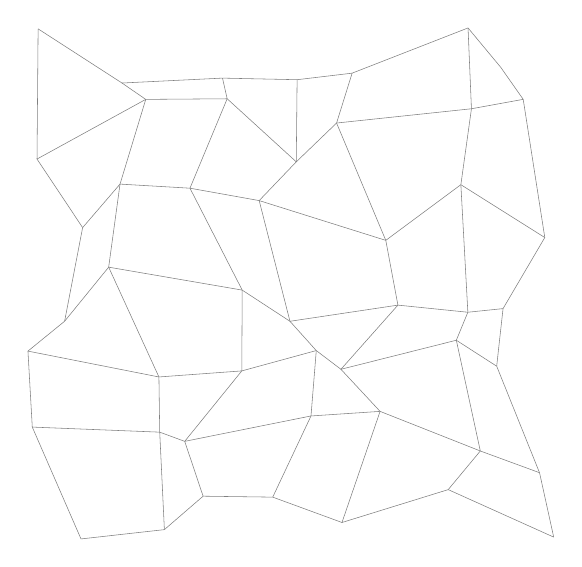
\begin{tikzpicture}
			\foreach \i [evaluate={\ii=int(\i-1);}] in {0,...,6}{
  			\foreach \j [evaluate={\jj=int(\j-1);}] in {0,...,6}{
    			\coordinate [shift={(\j,\i)}] (n-\i-\j) at (rand*190:1/3+rnd/8);
				\ifnum\i>0
  					\draw [help lines] (n-\i-\j) -- (n-\ii-\j);
				\fi
				\ifnum\j>0
  					\draw [help lines] (n-\i-\j) -- (n-\i-\jj);
				\fi
			}}
		\end{tikzpicture}
		\end{adjustbox}
	\caption{Malla no estructurada.}
	\end{subfigure}
	\caption{Tipos de mallas$^{\cite{Roda-Casanova2021}}$.}
	\label{mallas}
\end{figure}

\noindent
\justify

La conversi\'on de las ecuaciones diferenciales parciales requieren la discretizaci\'on del dominio de estudio; que, a su vez, depende de la dimensionalidad del problema.

\subsubsection{Solucionadores}

\noindent
\justify

Existen diferentes m\'etodos de soluci\'on de sistemas de ecuaciones algebraicas que pueden ser: \textit{exactos} o \textit{iterativos}. Los solucionadores que emplean m\'etodos exactos no suelen usarse en simulaciones num\'ericas debido al alto costo computacional. B\'asicamente tratan de resolver el sistema matricial $A \phi = B \rightarrow \phi = A^{-1} B$. 

\noindent
\justify

Los m\'etodos iterativos suelen basarse en la l\'ogica de \textit{suposici\'on} y \textit{corroboraci\'on}. El m\'etodo de Gauss - Seidel$^{\cite{Bai2021}}$, por ejemplo, inicia suponiendo el valor de una variable, corrobor\'andola con el c\'alculo de las dem\'as; en caso de no coincidir, su supone el resultado final de la variable supuesta, donde se vuelve a corroborar hasta que el supuesto y la corroboraci\'on coincidan o hasta que el margen de error sea tolerable.

\subsubsection{Metodolog\'ias de verificaci\'on y validaci\'on} \label{verified}

\noindent
\justify

Tienen por objetivo garantizar el menor \textit{error computacional} posible. Entre ellas se destacan:

\begin{itemize}
	\item \textit{Simple}: estudio de la evoluci\'on global o local de una variable debido al refinamiento de malla, como se aprecia en la Figura \ref{valsimple}.
	\begin{figure}[h!]
	\centering
	\begin{tikzpicture}
		\begin{axis}[
			domain = 0:1000,
			grid = both, minor tick num=2,
			title = \textbf{Validaci\'on por refinamiento de malla},
			xlabel = N\'umero de nodos,
			ylabel = Valor,
			legend pos = outer north east,
			restrict y to domain* = 0:100,
			width=10cm, height=8cm
		]
		\addplot[blue, line width=2pt] {\val};
		\addplot[
        scatter,scatter src=explicit symbolic,
        scatter/classes={
            a={mark=o,black},
            b={mark=triangle*,red},
            c={mark=o,draw=black,fill=black}
        }
    ]
    table[x=x,y=y,meta=label]{
        x	y	label
		10	30	a
		15	32	a
		30	43	a
		60	55	a
		100	70	a
		300	80	a
		600	92	a
		800	95	a
		1000	96	a

    };
		\legend{Te\'orico, Num\'erico};
		\end{axis}
	\end{tikzpicture}
	\caption{M\'etodo de validaci\'on simple.}
	\label{valsimple}
	\end{figure}
	\item \textit{Detallada}: se basa en la extrapolaci\'on generalizada de Richardson y en el \'indice de convergencia de malla (GCI).
	\item \textit{Experimentaci\'on}: se validan los resultados con estudios experimentales.
\end{itemize}

\subsubsection{An\'alisis bidimensional - 2D} \label{CFD2D}

\noindent
\justify

Para an\'alisis bidimensional, se busca resolver la Ecuaci\'on \ref{2DCFD}.

\begin{equation}
\underbrace{\rho \frac{\partial \phi}{\partial t}}_{\text{transitorio}} + \underbrace{\rho u \frac{\partial \phi}{\partial x} + \rho v \frac{\partial \phi}{\partial y}}_{\text{convectivo}} = \underbrace{ \frac{\partial}{\partial x} \left( \Gamma \frac{\partial \phi}{\partial x} \right) + \frac{\partial}{\partial y} \left( \Gamma \frac{\partial \phi}{\partial y} \right)}_{\text{difusivo}} + \underbrace{S_{\phi}}_{\text{fuente}}
\label{2DCFD}
\end{equation}

\noindent
\justify

La discretizaci\'on del dominio se realiza acorde a la Figura \ref{dis2D}.

\begin{figure}[h!]
\centering
\begin{tikzpicture}
\draw (0,0) rectangle (6,6);
\newcounter{contx} %counter
\setcounter{contx}{0}
\newcounter{conty} %counter
\setcounter{conty}{0}
\foreach \x in {0,1.5,3,4.5}
    \foreach \y in {0,1.5,3,4.5}
      {
        \draw (\x,\y) rectangle (\x + 1.5, \y + 1.5);
        \draw[fill=black] (\x + 0.75, \y + 0.75) circle (0.5mm);
        \stepcounter{conty}
        \ifnum \value{contx}<3
        	\draw[red, -triangle 90, fill=red] (\x+1.3, \y + 0.75) -- (\x+1.7, \y + 0.75);
        \fi
        \ifnum \value{conty}=4
        	\setcounter{conty}{0}
        	\stepcounter{contx}
        \else
        	\draw[blue, -triangle 90, fill=blue] (\x+0.75, \y + 1.3) -- (\x+0.75, \y + 1.7);
        \fi
      }

\foreach \x in {0,1.5,3,4.5}
	{
		\draw[fill=black] (\x + 0.75, 0) circle (0.5mm);
		\draw[fill=black] (\x + 0.75, 6) circle (0.5mm);
	}

\foreach \y in {0,1.5,3,4.5}
	{
		\draw[fill=black] (0, \y + 0.75) circle (0.5mm);
		\draw[fill=black] (6, \y + 0.75) circle (0.5mm);
	}

\node at (2.5,2.5) {P};
\node at (4,2.5) {E};
\node at (2.5,4) {N};
\node at (2.5,1) {S};
\node at (1,2.5) {W};

\end{tikzpicture}
\caption{Discretizaci\'on dominio bidimensional.}
\label{dis2D}
\end{figure}

\noindent
\justify

Existen diferentes enfoques para el an\'alisis de problemas bidimensionales, entre ellos se encuentran: diferencias centradas, \textit{upwind} e h\'ibrido. El acercamiento por diferencias centradas asume una variaci\'on lineal de $\phi$ entre nodos para una malla uniforme, de modo que:

\begin{equation}
\begin{array}{c}
	a_P \phi _P = a_E \phi _E  + a_W \phi _W + a_N \phi _N + a_S \phi _S + b \\
	a_E = D_e - F_e/2 \\
	a_W = D_w + F_w/2 \\
	a_N = D_n - F_n/2 \\
	a_S = D_s + F_s/2 \\
	a_P = a_E + a_W + a_N + a_S + \rho \frac{\Delta x \Delta y}{\Delta t} + \left(F_e - F_w + F_n - F_s \right) \\
	b = \rho \frac{\Delta x \Delta y}{\Delta t} \phi _P ^0 + S \Delta x \Delta y
\end{array}
\end{equation}

\subsection{M\'etodo de Elementos Discretos}


\noindent
\justify

El m\'etodo de elementos discretos (DEM) es un m\'etodo que modela fuerzas interpart\'icula basadas en par\'ametros de elasticidad y la superposici\'on de part\'iculas no deformadas, que se entiende como la cantidad de deformaci\'on necesaria para que puedan, f\'isicamente, ocupar el espacio en su actual configuraci\'on. Requiere de seis grados de libertad en cuerpos r\'igidos: tres en dos dimensiones y seis en tres dimensiones.

\begin{figure}[h!]
	\centering
	\includegraphics[width=\textwidth]{Images/DEM.PNG}
	\label{dem}
	\caption{Comparaci\'on entre metodolog\'ias de an\'alisis de part\'iculas para una esfera suave deformada en un plano: situaci\'on f\'isica real (izquierda), modelo analizado con el m\'etodo de elementos finitos (centro) y modelo con el m\'etodo de elementos discretos (derecha). Fuente: \v Smilauer 2015$^{\cite{Smilauer2015}}$.}
\end{figure}

\noindent
\justify

El principio de este m\'etodo es el de computar las fuerzas proporcionales a la superposici\'on geom\'etrica de las part\'iculas empleadas. Para part\'iculas esf\'ericas, o circulares, las fuerzas involucradas son de tipo central; a diferencia de otras configuraciones geom\'etricas, debido a que deben caracterizar las fuerzas en la forma `d\'ebil' y `fuerte'. 

\noindent
\justify

Una simulaci\'on que emplea este m\'etodo num\'erico, normalmente se rige bajo los siguientes pasos:

\begin{enumerate}
	\item Detecci\'on de colisi\'on entre part\'iculas.
	\item Creaci\'on de una nueva interacci\'on y determinaci\'on de diferentes propiedades, entre ellas la rigidez.
\end{enumerate}

\noindent
\justify

Para interacciones ya existentes:

\begin{enumerate}
	\item Evaluaci\'on de deformaci\'on.
	\item Computaci\'on del esfuerzo basada en la deformaci\'on.
	\item Aplicaci\'on de fuerzas en la interacci\'on entre part\'iculas.
\end{enumerate}

\subsubsection{Detecci\'on de una colici\'on} \label{detect}

\noindent
\justify

La detecci\'on \textit{exacta} de colisi\'on entre dos part\'iculas requiere de un alto costo computacional. Tomando una pareja de cuerpos $i$ y $j$ y su colisici\'on `exacta' (en el sentido de precisi\'on admisible por la implementaci\'on num\'erica) presentadas en los puntos $P_i$ y $P_j$ la detecci\'on procede en los siguientes dos puntos:

\begin{enumerate}
	\item Detecci\'on de colisi\'on r\'apida usando puntos aproximados $\widetilde{P}_i$ y $\widetilde{P}_j$; siendo estos preconstrucciones en el modo que caracter\'isticas individuales $P_i$ y $P_j$ satisfacen la siguiente condici\'on mostrada en la Ecuaci\'on \ref{cond}.
	\begin{equation}
		\forall x \in R^3 : x \in P_i \rightarrow x \in \widetilde{P}_i
		\label{cond}
	\end{equation}
	De igual manera para $P_j$. El predicado aproximaado se conoce como `volumen l\'imite', siguiendo lo siguiente:
	\begin{equation}
		\left(\widetilde{P}_i \cap \widetilde{P}_j \right) = {\O} \rightarrow \left( P_i \cap P_j \right) = {\O}
		\label{imposible}
	\end{equation}
	\item Al filtrar las colisiones imposibles mediante la Ecuaci\'on \ref{imposible}, algoritmos de detecci\'on de mayor costo computacional pueden ser impementados al filtrar falsas parejas de colisi\'on restantes, como se observa en la Figura \ref{colision}.
	\begin{equation}
		\left(\widetilde{P}_i \cap \widetilde{P}_j \right) \neq {\O} \wedge \left(P_i \cap P_j \right) = {\O}
	\end{equation}
\end{enumerate}

\begin{figure}[h!]
\centering
\includegraphics[width=0.9\textwidth]{Images/Colision.PNG}
\caption{Detecci\'on de colisi\'on entre part\'iculas. Fuente: \v Smilauer 2015$^{\cite{Smilauer2015}}$.}
\label{colision}
\end{figure}

\noindent
\justify

Yade$^{\cite{Smilauer2015}}$ emplea un algoritmo conocido como ``\texttt{Aabb}" (\textit{Caja de contorno para alineaci\'on de eje}, por sus siglas en ingl\'es); visualmente, consisten en los rect\'angulos de contorno que rodean cada esfera de la Figura \ref{colision}. Cada caja de contorno es usada como $\widetilde{P}_i$; estando definida cada una por sus esquinas $\varepsilon R^3$ siendo $\widetilde{P}_i ^{x0}$ y $\widetilde{P}_i ^{x1}$ las coordenadas en el eje $x$ de la esfera $P_1$, por ejemplo. 

\noindent
\justify

La presencia de superposici\'on entre part\'iculas entre dos \texttt{Aabb}'s se determina mediante el conjunto de superposici\'on separada de intervalos sobre cada eje. Est\'a representada por la Ecuaci\'on \ref{overlap:dem}.

\begin{equation}
	\left(\widetilde{P}_i \cap \widetilde{P}_j \right) \neq {\O} \Longleftrightarrow \bigwedge_{w \epsilon \{x,y,z \}} \left[\left(\left(\widetilde{P}_i ^{w0}, \widetilde{P}_i ^{w1} \right) \cap \left(\widetilde{P}_j ^{w0}, \widetilde{P}_j ^{w1} \right) \right) \neq {\O} \right] 
	\label{overlap:dem}
\end{equation}

\begin{center}
	\section{CFD-DEM}
\end{center}

\noindent
\justify

En el acoplamiento cl\'asico entre CFD-DEM, el flujo se resuelve a trav\'e del m\'etodo CFD basado en malla, mientras que la fase s\'olida es modelada mediante DEM para cada part\'icula sujeta a trav\'es de fuerzas hidrodin\'amicas, fuerzas de cuerpo (como la gravedad) y a trav\'es de fuerzas de contacto, actualizando valores de velocidad y posici\'on conforme a la segunda ley de Newton (Hoomans \textit{et al.}, 1996; Tsuji \textit{et al.}, 1993; Xu y Yu, 1997). En principio, todos los m\'etodos CFD pueden acoplarse con DEM; lo que ha dado origen a diferentes m\'etodos discretos y continuos, tal como el m\'etodo de Lattice Boltzmann (LBM), Hidrodin\'amica de Part\'iculas Suaves (SPH), m\'etodos de Diferencias Finitas y Vol\'umenes Finitos (FVM).

\noindent
\justify

Gran parte de las simulaciones reportadas en la literatura comprenden modelos 2D o sistemas prototipados de peque\~na escala. En busca de acelerar los tiempos de simulaci\'on e incrementar la eficiencia computacional, se han desarrollado t\'ecnicas de computaci\'on paralela; donde gran parte de los esfuerzos han sido enfocados en la paralelizaci\'on del DEM. Muchos algoritmos se han propuesto para lograr este hecho, como la t\'ecnica de espejo de dominio (Damana, \textit{et al.}, 2006; Washington y Meegoda, 2003), el m\'etodo de subconjunto de part\'iculas (Kafui \textit{et al.}, 2011) y m\'etodos de descomposici\'on de dominios (Amritkar \textit{et al.}, 2014; Tsuji \textit{et al.}, 2008). El uso de estos algoritmos depende de la arquitectura del hardware. La paralelizaci\'on sobre memoria compartida del sistema se alcanza, normalmente, empleando \textit{OpenMP} (``Open Multi-Processing", por sus siglas en ingl\'es), mientras que el MPI (Interfaz de Paso de Mensajes) se emplea en sistemas de memoria distirbuida (Rabenseifner \textit{et al.}, 2009). Por ejemplo, Tsuji \textit{et al.} (2008) paralelizaron una simulaci\'on en CFD-DEM usando MPI para el intercambio de informaci\'on entre 16 CPUs, reportando el comportamiento fluidodin\'amico de 4.5 millones de part\'iculas en un medio gaseoso; empleando el m\'etodo unidimensional de descomposici\'on de dominio.

\subsection{Fase del solvente}

\noindent
\justify

En un modelo CFD-DEM, la fase del fluido se resuleve en el nivel computacional en cada elemento de la malla (ver Figura \ref{elemento}) empleando un marco de referencia Euleriano mientras que el movimiento de la part\'icula se sigue a trav\'es de un marco de referencia Lagrangiano. Para lograr el acoplamiento de fase, es necesario interpolar las propiedades de las part\'iculas a los centroides de los elementod CFD y las propiedades del fluido a la posici\'on de cada part\'icula. Como se muestra en la Figura \ref{particle}, se crean dos mallas alineadas de b\'usqueda: la malla de b\'usqueda de part\'iculas (amarilla) y la malla de b\'usqueda de fluido (azul). 

\begin{figure}[h!]
	\centering
	\begin{subfigure}[b]{0.3\textwidth}
		\centering
		\begin{adjustbox}{max width = \textwidth}
		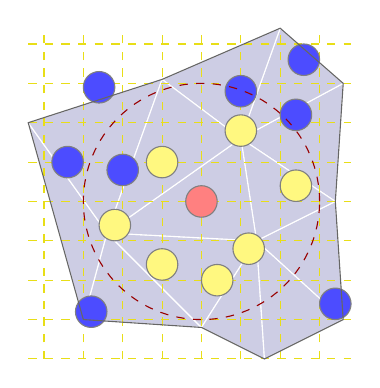
\begin{tikzpicture}
		%---Interno---
	%1 - (-1.2, -0.4)
	\draw[white, fill=blue!30!gray!30!white] (-1.5, -1.5) -- (0,-1.6) -- (-1.2, -0.4) -- cycle;
	\draw[white, fill=blue!30!gray!30!white] (-2.2, 1) -- (-1.5,-1.5) -- (-1.2, -0.4) -- cycle;
	\draw[white, fill=blue!30!gray!30!white] (-2.2, 1) -- (-0.5, 1.55) -- (-1.2, -0.4) -- cycle;
	%2 - (0.7, -0.5)
	\draw[white, fill=blue!30!gray!30!white] (-1.2, -0.4) -- (0,-1.6) -- (0.7, -0.5) -- cycle;
	\draw[white, fill=blue!30!gray!30!white] (0.8,-2) -- (0,-1.6) -- (0.7, -0.5) -- cycle;
	\draw[white, fill=blue!30!gray!30!white] (1.8,-1.5) -- (0.8,-2) -- (0.7, -0.5) -- cycle;
	\draw[white, fill=blue!30!gray!30!white] (1.8,-1.5) -- (1.7,0) -- (0.7, -0.5) -- cycle;
	%3 - (0.5,0.8)
	\draw[white, fill=blue!30!gray!30!white] (1.7,0) -- (1.8,1.5) -- (0.5, 0.8) -- cycle;
	\draw[white, fill=blue!30!gray!30!white] (1.7,0) -- (0.7, -0.5) -- (0.5, 0.8) -- cycle;
	\draw[white, fill=blue!30!gray!30!white] (1,2.2) -- (1.8,1.5) -- (0.5, 0.8) -- cycle;
	\draw[white, fill=blue!30!gray!30!white] (-0.5,1.55) -- (1,2.2) -- (0.5, 0.8) -- cycle;
	\draw[white, fill=blue!30!gray!30!white] (-1.2,-0.4) -- (0.7,-0.5) -- (0.5, 0.8) -- cycle;
	\draw[white, fill=blue!30!gray!30!white] (-1.2,-0.4) -- (-0.5,1.55) -- (0.5, 0.8) -- cycle;
	
	%malla
	\draw[step=0.5, dashed, yellow!90!black] (-2.2, -2) grid (1.9,2.2);
	
	%Partículas
	\draw[black!50, fill=red!50] (0,0) circle (2mm);
	\draw[black!50, fill=yellow!50] (0.6,-0.6) circle (2mm);
	\draw[black!50, fill=yellow!50] (-1.1,-0.3) circle (2mm);
	\draw[black!50, fill=yellow!50] (0.5,0.9) circle (2mm);
	\draw[black!50, fill=yellow!50] (-0.5,0.5) circle (2mm);
	\draw[black!50, fill=yellow!50] (1.2,0.2) circle (2mm);
	\draw[black!50, fill=yellow!50] (-0.5,-0.8) circle (2mm);
	\draw[black!50, fill=yellow!50] (0.2,-1) circle (2mm);
	
	\draw[black!50, fill=blue!70] (1.7,-1.3) circle (2mm);
	\draw[black!50, fill=blue!70] (-1.4,-1.4) circle (2mm);
	\draw[black!50, fill=blue!70] (-1,0.4) circle (2mm);
	\draw[black!50, fill=blue!70] (-1.7, 0.5) circle (2mm);
	\draw[black!50, fill=blue!70] (-1.3,1.45) circle (2mm);
	\draw[black!50, fill=blue!70] (1.2, 1.1) circle (2mm);
	\draw[black!50, fill=blue!70] (0.5,1.4) circle (2mm);
	\draw[black!50, fill=blue!70] (1.3,1.8) circle (2mm);
	
	%Carcasa
	\draw[black!60] (-2.2, 1) -- (-0.5, 1.55) -- (1, 2.2) -- (1.8, 1.5) -- (1.7, 0) -- (1.8, -1.5) -- (0.8, -2) -- (0, -1.6) -- (-1.5, -1.5) -- cycle;
	 
	 %Círculo rojo
	\draw[red!60!black, dashed] (0,0) circle (1.5 cm);
		\end{tikzpicture}
		\end{adjustbox}
		\caption{B\'usqueda de part\'iculas vecinas y c\'alculo de la fracci\'on de vac\'io de una part\'icula dada.}
	\end{subfigure}
	\hfill
	\begin{subfigure}[b]{0.3\textwidth}
		\centering
		\begin{adjustbox}{max width = \textwidth}
		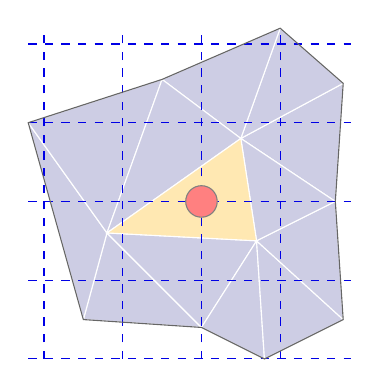
\begin{tikzpicture}
		%---Interno---
	%1 - (-1.2, -0.4)
	\draw[white, fill=blue!30!gray!30!white] (-1.5, -1.5) -- (0,-1.6) -- (-1.2, -0.4) -- cycle;
	\draw[white, fill=blue!30!gray!30!white] (-2.2, 1) -- (-1.5,-1.5) -- (-1.2, -0.4) -- cycle;
	\draw[white, fill=blue!30!gray!30!white] (-2.2, 1) -- (-0.5, 1.55) -- (-1.2, -0.4) -- cycle;
	%2 - (0.7, -0.5)
	\draw[white, fill=blue!30!gray!30!white] (-1.2, -0.4) -- (0,-1.6) -- (0.7, -0.5) -- cycle;
	\draw[white, fill=blue!30!gray!30!white] (0.8,-2) -- (0,-1.6) -- (0.7, -0.5) -- cycle;
	\draw[white, fill=blue!30!gray!30!white] (1.8,-1.5) -- (0.8,-2) -- (0.7, -0.5) -- cycle;
	\draw[white, fill=blue!30!gray!30!white] (1.8,-1.5) -- (1.7,0) -- (0.7, -0.5) -- cycle;
	%3 - (0.5,0.8)
	\draw[white, fill=blue!30!gray!30!white] (1.7,0) -- (1.8,1.5) -- (0.5, 0.8) -- cycle;
	\draw[white, fill=blue!30!gray!30!white] (1.7,0) -- (0.7, -0.5) -- (0.5, 0.8) -- cycle;
	\draw[white, fill=blue!30!gray!30!white] (1,2.2) -- (1.8,1.5) -- (0.5, 0.8) -- cycle;
	\draw[white, fill=blue!30!gray!30!white] (-0.5,1.55) -- (1,2.2) -- (0.5, 0.8) -- cycle;
	\draw[white, fill=blue!30!gray!30!white] (-1.2,-0.4) -- (-0.5,1.55) -- (0.5, 0.8) -- cycle;
	\draw[white, fill=red!30!yellow!30!white] (-1.2,-0.4) -- (0.7,-0.5) -- (0.5, 0.8) -- cycle;
	
	%malla
	\draw[step=1, dashed, blue!90!black] (-2.2, -2) grid (1.9,2.2);
	
	%Partículas
	\draw[black!50, fill=red!50] (0,0) circle (2mm);
	
	%Carcasa
	\draw[black!60] (-2.2, 1) -- (-0.5, 1.55) -- (1, 2.2) -- (1.8, 1.5) -- (1.7, 0) -- (1.8, -1.5) -- (0.8, -2) -- (0, -1.6) -- (-1.5, -1.5) -- cycle;
	 
		\end{tikzpicture}
		\end{adjustbox}
	\caption{Mapeo de una part\'icula dada dentro del fluido para interpolar sus propiedades en ese punto.}
	\end{subfigure}
	\hfill
	\begin{subfigure}[b]{0.3\textwidth}
		\centering
		\begin{adjustbox}{max width = \textwidth}
		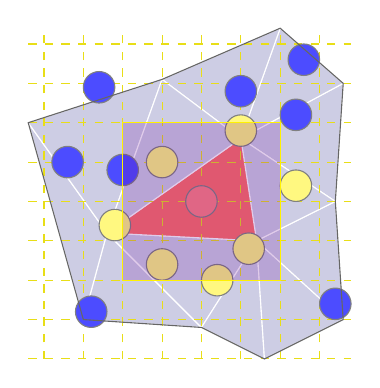
\begin{tikzpicture}
		%---Interno---
	%1 - (-1.2, -0.4)
	\draw[white, fill=blue!30!gray!30!white] (-1.5, -1.5) -- (0,-1.6) -- (-1.2, -0.4) -- cycle;
	\draw[white, fill=blue!30!gray!30!white] (-2.2, 1) -- (-1.5,-1.5) -- (-1.2, -0.4) -- cycle;
	\draw[white, fill=blue!30!gray!30!white] (-2.2, 1) -- (-0.5, 1.55) -- (-1.2, -0.4) -- cycle;
	%2 - (0.7, -0.5)
	\draw[white, fill=blue!30!gray!30!white] (-1.2, -0.4) -- (0,-1.6) -- (0.7, -0.5) -- cycle;
	\draw[white, fill=blue!30!gray!30!white] (0.8,-2) -- (0,-1.6) -- (0.7, -0.5) -- cycle;
	\draw[white, fill=blue!30!gray!30!white] (1.8,-1.5) -- (0.8,-2) -- (0.7, -0.5) -- cycle;
	\draw[white, fill=blue!30!gray!30!white] (1.8,-1.5) -- (1.7,0) -- (0.7, -0.5) -- cycle;
	%3 - (0.5,0.8)
	\draw[white, fill=blue!30!gray!30!white] (1.7,0) -- (1.8,1.5) -- (0.5, 0.8) -- cycle;
	\draw[white, fill=blue!30!gray!30!white] (1.7,0) -- (0.7, -0.5) -- (0.5, 0.8) -- cycle;
	\draw[white, fill=blue!30!gray!30!white] (1,2.2) -- (1.8,1.5) -- (0.5, 0.8) -- cycle;
	\draw[white, fill=blue!30!gray!30!white] (-0.5,1.55) -- (1,2.2) -- (0.5, 0.8) -- cycle;
	\draw[white, fill=red!95!yellow!60!white] (-1.2,-0.4) -- (0.7,-0.5) -- (0.5, 0.8) -- cycle;
	\draw[white, fill=blue!30!gray!30!white] (-1.2,-0.4) -- (-0.5,1.55) -- (0.5, 0.8) -- cycle;
	
	%malla
	\draw[step=0.5, dashed, yellow!90!black] (-2.2, -2) grid (1.9,2.2);
	
	%Partículas
	\draw[black!50, fill=red!50] (0,0) circle (2mm);
	\draw[black!50, fill=yellow!50] (0.6,-0.6) circle (2mm);
	\draw[black!50, fill=yellow!50] (-1.1,-0.3) circle (2mm);
	\draw[black!50, fill=yellow!50] (0.5,0.9) circle (2mm);
	\draw[black!50, fill=yellow!50] (-0.5,0.5) circle (2mm);
	\draw[black!50, fill=yellow!50] (1.2,0.2) circle (2mm);
	\draw[black!50, fill=yellow!50] (-0.5,-0.8) circle (2mm);
	\draw[black!50, fill=yellow!50] (0.2,-1) circle (2mm);
	
	\draw[black!50, fill=blue!70] (1.7,-1.3) circle (2mm);
	\draw[black!50, fill=blue!70] (-1.4,-1.4) circle (2mm);
	\draw[black!50, fill=blue!70] (-1,0.4) circle (2mm);
	\draw[black!50, fill=blue!70] (-1.7, 0.5) circle (2mm);
	\draw[black!50, fill=blue!70] (-1.3,1.45) circle (2mm);
	\draw[black!50, fill=blue!70] (1.2, 1.1) circle (2mm);
	\draw[black!50, fill=blue!70] (0.5,1.4) circle (2mm);
	\draw[black!50, fill=blue!70] (1.3,1.8) circle (2mm);
	
	%Carcasa
	\draw[black!60] (-2.2, 1) -- (-0.5, 1.55) -- (1, 2.2) -- (1.8, 1.5) -- (1.7, 0) -- (1.8, -1.5) -- (0.8, -2) -- (0, -1.6) -- (-1.5, -1.5) -- cycle;
	
	\draw[yellow, fill=red!40!blue, fill opacity=0.2] (-1,-1) rectangle (1,1);
		\end{tikzpicture}
		\end{adjustbox}
	\caption{Mapeo del elemento de malla CFD para el c\'alculo de t\'erminos fuente en el elemento de inter\'es.}
	\end{subfigure}
	\caption{Esquema de la aproximaci\'on por malla dual para la b\'usqueda de part\'iculas vecinas en un fluido.}
	\label{particle}
\end{figure}

\noindent
\justify

Los pasos clave con los que se basan las mallas de b\'usqueda son: detecci\'on de colisi\'on de part\'iculas (descrito en la secci\'on \ref{detect}), geometr\'ia de los elementos de malla CFD (detallado en la secci\'on \ref{CFD2D}) y el c\'alculo de fuerzas de fluido, entre otras.

\noindent
\justify

Para el c\'alculo de las fuerzas ejercidas por el fluido, se requiere conocer las propiedades del fluido en la posici\'on de la part\'icula; incluyendo el gradiente de presi\'on, la velocidad del flujo y el gradiente de velocidades (para fluidos gaseosos). Normalmente, las propiedades del fluido se `almacenan' en el centroide de los elementos de malla durante c\'alculos mediante FVM, como se muestra en la Ecuaci\'on \ref{properties}.

\begin{equation}
\phi _p = \phi _{el} + \nabla \phi _{el} \cdot r_{pc}
\label{properties}
\end{equation}

\noindent
\justify

D\'onde: $\phi _p$ y $\phi _{el}$ son las propiedades del fluido en la posici\'on de la part\'icula y el centroide del elemento, respectivamente; y $r_{pc}$ es el vector distancia que va desde el centro del elemento hasta la posici\'on de la part\'icula. 

\begin{center}
	\section{Sedimentaci\'on}
\end{center}

\noindent
\justify

Se plantea que el \textit{principio funcional} del sistema de eluci\'on y filtrado de la planta de extracci\'on recaiga sobre este fen\'omeno natural.

\noindent
\justify

Los tanques de sedimentaci\'on han sido ampliamente usados como medios filtrantes en plantas purificadoras de agua debido a su capacidad de remoci\'on de residuos s\'olidos; siendo empleadas para limpiar aguas con turbidez\footnote{La turbidez define el nivel de transparencia de fluidos incoloros en contraste a la presencia de part\'iculas en suspensi\'on.} de hasta $50 [NTU]^{\cite{Voutchkov2017}}$\footnote{La Organizaci\'on Mundial de la Salud estipula que el agua de consumo humano debe presentar un nivel de turbidez inferior a $2 [NTU]^{\cite{OMSagua}}$.}. 

\noindent
\justify

Para asegurar un correcto nivel de turbidez, los sistemas de sedimentaci\'on convencionales emplean coagulantes (normalmente sales de hierro) y floculantes (pol\'imeros) en el sistema de alimentaci\'on. Cuando el fluido excede el nivel de $50 [NTU]$, se recomienda emplear sistemas de sedimentaci\'on de placas inclinadas$^{\cite{Voutchkov2017}}$ para la remoci\'on de elementos s\'olidos de bajo tama\~no de part\'icula.


\subsection{Sedimentadores convencionales}

\noindent
\justify

Son ampliamente usados para la remoci\'on de part\'iculas en fluidos con turbidez de $20 [NTU]^{\cite{Voutchkov2017}}$. Consiste de un sistema de una sola etapa estructurado de forma circular o rectangular. A la fecha, sedimentadores rectangulares se emplean sistemas de pretratamiento de aguas salinas por su bajo costo de inversi\'on y gran desempe\~no. Los par\'ametros clave para el dise\~no de estos sistemas son los siguientes:

\begin{itemize}
	\item N\'umero m\'inimo de tanques: 4
	\item Produndidad del agua: $3.0 - 4.0 [m]$.
	\item Velocidad media de flujo: $0.3 - 1.1 [m/min]$.
	\item Tiempo de detenci\'on: $2 - 4 [h]$.
	\item Relaci\'on ancho-largo: m\'inimo de 4:1.
	\item Relaci\'on profundidad-largo: m\'inimo de 1:15 
	\item Velocidad del recolector de lodos: $0.4 - 0.8 [m/min]$.
\end{itemize}

\newpage

\subsection{Sedimentador de placas inclinadas}

\noindent
\justify

Estos tanques de sedimentaci\'on, tambi\'en conocidos como \textit{clarificadores}, tienen un desempe\~no altamente superior a los convencionales, llegando a clarificar fluidos de hasta $200 [NTU]^{\cite{Voutchkov2017}}$ de turbidez. Normalmente tienen una estructura rectangular o circular y son ampliamente usados para la limpieza de agua marina. 

\begin{figure}[h!]
	\centering
	\includegraphics[width=\textwidth]{Images/lamelas_inclinadas.png}
	\caption{Esquema de un sedimentador de placas inclinadas$^{\cite{Voutchkov2017}}$.}
	\label{lamelas_inclinadas}
\end{figure}


\noindent
\justify

Los criterios clave de dise\~no para su uso en plantas de trateminto de agua se evidencia a continuaci\'on:

\begin{itemize}
	\item N\'umero m\'inimo de tanques: 2
	\item Produndidad del agua: $3.5 - 5.0 [m]$.
	\item Velocidad media de flujo: $0.3 - 1.1 [m/min]$.
	\item Tiempo de detenci\'on: $0.2 - 0.4 [h]$.
	\item Velocidad del recolector de lodos: $0.4 - 0.8 [m/min]$.
\end{itemize}

\subsubsection{Desarrollo te\'orico} \label{Acribos}

\noindent
\justify

Considere el caso bidimensional mostrado en la Figura \ref{teo_sed} que consiste de una superficie de longitud infinita y ancho arbitrario, inclinada a un \'angulo $\theta$ sobre la horizontal y ubicada en una suspensi\'on infinita de esferas pesadas de radio $\tilde{a}$. La fracci\'on de volumen de las part\'iculas, tambi\'en conocido como la alimentaci\'on de part\'iculas, se identifica mediante el s\'imbolo $\phi _s$.

\newcommand\ang{45}
\newcommand\aancho{2}
\newcommand\LL{7.5}


\begin{figure}[h!]
	\centering
	\begin{tikzpicture}
		%Lamela
		\draw (0,0) -- ({\aancho*cos(90-\ang)},{\aancho*sin(90-\ang)});
		\draw[line width=1.0mm] (0,0) -- ({-\LL*cos(\ang)}, {\LL*sin(\ang)});
		\draw ({-\LL*cos(\ang)}, {\LL*sin(\ang)}) -- ({-\LL*cos(\ang)+\aancho*cos(90-\ang)}, {\LL*sin(\ang) + \aancho*sin(90-\ang)});
		\draw[line width=1.0mm] ({-\LL*cos(\ang)+\aancho*cos(90-\ang)}, {\LL*sin(\ang) + \aancho*sin(90-\ang)}) -- ({\aancho*cos(90-\ang)},{\aancho*sin(90-\ang)});
		
		%--Medidas--
		%b
		\draw ({0.25*cos(\ang)}, {-0.25*sin(\ang)}) -- ({0.5*cos(\ang)}, {-0.5*sin(\ang)});
		\draw ({\aancho*cos(90-\ang) + 0.25*cos(\ang)},{\aancho*sin(90-\ang) - 0.25*sin(\ang)}) -- ({\aancho*cos(90-\ang) + 0.5*cos(\ang)},{\aancho*sin(90-\ang) - 0.5*sin(\ang)});	
		
		\draw[-triangle 45, fill=black] ({0.375*cos(\ang)}, {-0.375*sin(\ang)}) -- ({\aancho*cos(90-\ang) + 0.375*cos(\ang)},{\aancho*sin(90-\ang) - 0.375*sin(\ang)});

		\draw[-triangle 45, fill=black] ({\aancho*cos(90-\ang) + 0.375*cos(\ang)},{\aancho*sin(90-\ang) - 0.375*sin(\ang)}) -- ({0.375*cos(\ang)}, {-0.375*sin(\ang)}) node [midway, below, rotate=\ang] {$b$};	
		
		%L
		\draw ({-0.25*cos(\ang)}, {-0.25*sin(\ang)}) -- ({-0.5*cos(\ang)}, {-0.5*sin(\ang)});
		
		\draw ({-0.8*\LL*cos(\ang)-0.25*cos(\ang)}, {0.8*\LL*sin(\ang)-0.25*sin(\ang)}) -- ({-0.8*\LL*cos(\ang)-0.5*cos(\ang)}, {0.8*\LL*sin(\ang)-0.5*sin(\ang)});
		
		\draw[-triangle 45, fill=black] ({-0.375*cos(\ang)}, {-0.375*sin(\ang)}) -- ({-0.8*\LL*cos(\ang)-0.375*cos(\ang)}, {0.8*\LL*sin(\ang)-0.375*sin(\ang)});
		
		\draw[-triangle 45, fill=black] ({-0.8*\LL*cos(\ang)-0.375*cos(\ang)}, {0.8*\LL*sin(\ang)-0.375*sin(\ang)}) -- ({-0.375*cos(\ang)}, {-0.375*sin(\ang)}) node [midway, below, rotate=-\ang] {$L (t)$};
		
		%Theta
		\draw[dashed] (-0.75,0) -- (-0.3*\LL, 0);
		
		\draw (-0.15*\LL,0) arc (180:180-\ang:0.15*\LL) node [midway, left] {$\theta$};
		
		%H
		\draw (-0.775*\LL,0) -- (-0.825*\LL,0);
		\draw (-0.775*\LL,{0.8*\LL*sin(\ang)}) -- (-0.825*\LL,{0.8*\LL*sin(\ang)});
		
		\draw[-triangle 45, fill=black] (-0.8*\LL,0) -- (-0.8*\LL, {0.8*\LL*sin(\ang)});
		
		\draw[-triangle 45, fill=black] (-0.8*\LL, {0.8*\LL*sin(\ang)}) -- (-0.8*\LL,0) node [midway, right] {$H (t)$};
		
		%--Volúmenes--
		%Intermedio - oscure
		\draw[pattern=north west lines, pattern color=blue!40!black] (0,0) -- ({-0.85*\LL*cos(\ang)}, {0.85*\LL*sin(\ang)}) -- ({-0.6*\LL*cos(\ang) + 0.85*\aancho*cos(90-\ang)}, {0.6*\LL*sin(\ang) + 0.85*\aancho*sin(90-\ang)}) -- ({\aancho*cos(\ang)}, {\aancho*sin(\ang)}) -- cycle;
		
		%Claro
		\draw[pattern=dots, pattern color=blue!35!white] ({-0.85*\LL*cos(\ang)}, {0.85*\LL*sin(\ang)}) -- ({-\LL*cos(\ang)}, {\LL*sin(\ang)}) -- ({-\LL*cos(\ang)+\aancho*cos(90-\ang)}, {\LL*sin(\ang) + \aancho*sin(90-\ang)}) -- ({\aancho*cos(90-\ang)},{\aancho*sin(90-\ang)}) -- ({-0.6*\LL*cos(\ang) + 0.85*\aancho*cos(90-\ang)}, {0.6*\LL*sin(\ang) + 0.85*\aancho*sin(90-\ang)}) -- cycle;
		
		%Oscuro
		\draw[pattern=north east lines, pattern color=brown!80!gray] (0,0) -- ({0.2*\aancho*cos(90-\ang)},{0.2*\aancho*sin(90-\ang)}) -- ({-0.85*\LL*cos(\ang)}, {0.85*\LL*sin(\ang)}) -- cycle;
		
		
	\end{tikzpicture}
	\caption{An\'alisis de una lamela.}
	\label{teo_sed}
\end{figure}

\noindent
\justify

Acrivos$^{\cite{Acrivos1995}}$ model\'o la suspensi\'on como un fluido Newtoniano con propiedades f\'isicas \textit{efectivas} que, relativo a la propiedad correspondiente del l\'iquido suspendido, son funciones \'unicamente de la fracci\'on de volumen local de las part\'iculas. De esta manera, la densidad efectiva est\'a definida mediante la Ecuaci\'on \ref{rhoEff}.

\begin{equation}
	\tilde{\rho} (\phi) = \tilde{\rho} _f \, \gamma (\phi)
	\label{rhoEff}
\end{equation}

\noindent
\justify

De igual modo, la viscosidad efectiva se define de la siguiente manera:

\begin{equation}
	\tilde{\mu} (\phi) = \tilde{\mu} _f \, \lambda (\phi)
	\label{viscEff}
\end{equation}

\noindent
\justify

De las Ecuaciones \ref{rhoEff} y \ref{viscEff}: $\phi$ denota la fracci\'on de volumen local de las part\'iculas, la acentuaci\'on es un indicativo de que la variable en cuesti\'on presenta dimensiones y el suscrito $f$ se refiere a la propiedad correspondiente del fluido. En vista de esta descripci\'on continua efectiva, el balance de momento para el flujo suspendido puede escribirse de la forma usual, como se aprecia en la Ecuaci\'on \ref{generalSedT}.

\begin{equation}
	\frac{\partial}{\partial y} \left[ \lambda (\phi) \frac{\partial u}{\partial y} \right] + \frac{9}{2} \left( \phi - \phi _s \right) \sin \theta = R_p \, \gamma (\phi) \left( u \frac{\partial u}{\partial x} + v \frac{\partial u}{\partial y} \right)
	\label{generalSedT}
\end{equation}

\noindent
\justify

Siendo:

\begin{equation}
	\frac{\partial u}{\partial x} + \frac{\partial v}{\partial y} = 0
	\label{vels}
\end{equation}

\noindent
\justify

D\'onde: $\tilde{u} _t = \frac{2}{9} \tilde{a} ^2 \left( \tilde{\rho} _s - \tilde{\rho} _f \right)$ es la velocidad de asentamiento de Stokes del fluido l\'impio; $\tilde{\rho} _s$ es la densidad del s\'olido, de forma esf\'erica, y $R_p = \tilde{\rho} _f \, \tilde{u} _t \, \tilde{a} / \tilde{\mu} _f$ es el n\'umero de Reynolds de la part\'icula basada en el movimiento relativo entre la part\'icula y el fluido. Dado que $R_p$ es generalmente peque\~no en la mayor\'ia de sistemas pr\'acticos, el t\'ermino derecho de la Ecuaci\'on \ref{generalSedT} es despreciable \textit{dentro} de la capa de sedimentos (ver Figura \ref{teo_sed}). Adicionalmente, al aplicar el balance de momento en la direcci\'on $y$, la ca\'ida de presi\'on sobre la delgada capa es, tambi\'en, despreciable para esta aproximaci\'on.

\noindent
\justify

La presencia de cortante en una suspensi\'on concentrada induce a la migraci\'on de part\'iculas dentro de esta; la cual, junto con el flujo de sedimentos y el flujo a granel, tiende al desarrollo de concentraci\'on particular no uniforme, $\phi$. Para determinar este perfil, Acrivos$^{\cite{Acrivos1995}}$ explica que es necesario analizar, en adici\'on a la Ecuaci\'on de momento \ref{generalSedT}, la Ecuaci\'on de balance estable de part\'iculas.

\begin{equation}
	u \frac{\partial \phi}{\partial x} + v \frac{\partial \phi}{\partial y} + \frac{\partial}{\partial y} \left( N_g \right) + \frac{\partial}{\partial y} \left(N _d \right) = 0
	\label{balEs}
\end{equation}

\noindent
\justify

D\'onde $N_g$ y $N_d$ denotan, respectivamente, el flujo adimensional de part\'iculas debido al asentamiento gravitacional y al cortante inducido por la difusi\'on en la direcci\'on $y$.

\noindent
\justify

Las condiciones de frontera en $y=0$ son:

\begin{equation}
	v = 0
\end{equation}
	
\begin{equation}
	\left[\beta (\phi ) \frac{\partial u}{\partial y} \frac{\partial \phi}{\partial y} + \frac{\alpha (\phi )}{\lambda (\phi )} \frac{\partial}{\partial y} \left( \lambda (\phi ) \frac{\partial u}{\partial y} \right) \right] + \phi f (\phi ) \cos \theta = 0
	\label{bulto}
\end{equation}

\noindent
\justify

La Ecuaci\'on \ref{bulto} refleja que el flujo de sedimentaci\'on de las part\'iculas debe estar balanceado por su correspondiente flujo cortante difusivo si el flujo neto de part\'iculas en el muro est\'a por desaparecer; previniendo que la concentraci\'on de part\'iculas en el muro alcance su m\'aximo valor.

\noindent
\justify

Para el an\'alisis de la condici\'on de deslizamiento en el muro (zona de sedimentos), se emplea lo siguiente:

\begin{equation}
	u = \zeta \left( \partial u / \partial y \right) _{y=0} \, \text{en } \, y=0 
\end{equation}

\noindent
\justify

D\'onde $\zeta$ es el coeficiente de deslizamiento. Para una primera aproximaci\'on, se asume este coeficiente como una funci\'on de la fracci\'on de volumen particular sobre el muro.

\noindent
\justify

Acrivos$^{\cite{Acrivos1995}}$ compar\'o la soluci\'on del sistema de ecuaciones diferenciales parciales planteadas, resuelto mediante el m\'etodo de diferencias finitas, con los resultados experimentales referentes al espesor de la zona de sedimentos; reportando una diferencia media superior al $14 \%$ con respecto al modelo en donde se emplea la condici\'on de deslizamiento.

\subsubsection{Modelo simplificado} \label{simplificado}

\noindent
\justify

El modelo te\'orico expuesto en la secci\'on \ref{Acribos} estudia el sistema en estado \textit{estacionario} en una lamela y aproxima el flujo de sedimentos a un fluido denso y viscoso; contrario a la naturaleza propia del problema. Desde este enfoque, no es posible predecir la interacci\'on fluido-part\'icula durante la separaci\'on de las fases s\'olida y l\'iquida. Adicional al hecho de que este modelo te\'orico no presenta un nivel de precisi\'on lo suficientemente alto para definir un dise\~no final del sistema de sedimentaci\'on. Se expone, a continuaci\'on, una metodolog\'ia de dise\~no simplificada que permite proponer una geometr\'ia inicial, para su respectiva evaluaci\'on mediante el m\'etodo CFD-DEM.


\paragraph{An\'alisis hidrodin\'amico de una part\'icula} \label{hidroD}

\noindent
\justify

La \textit{sedimentaci\'on discreta} se refiere a un modelo de sedimentaci\'on en donde las part\'iculas s\'olidas no tienden a aglomerarse ni a colisionar entre s\'i. El comportamiento de los s\'olidos se encuentra, \'unicamente, en funci\'on de las propiedades de las part\'iculas y del fluido directamente. El balance de fuerzas sobre una part\'icula se puede apreciar directamente en la Figura \ref{partF}.

\begin{figure}[h!]
	\centering
	\begin{tikzpicture}
		\draw[pattern = dots, pattern color= brown] (0,0) circle (2);
		\node[align=center] at (0,0) {Spherical\\ particle};
		\draw[-triangle 45, gray!30!black] (0,3) node [above] {$\vec{W}$} -- (0,0.5) ;
		\foreach \x in {0, ..., 10}
			\draw[-triangle 45, blue!70!white] (0.4*\x-2,{-sqrt(2^2-(0.4*\x-2)^2)-0.5}) -- (0.4*\x-2,{-sqrt(2^2-(0.4*\x-2)^2)});
		\foreach \x in {0, ..., 10}
			\draw[-triangle 45, blue!70!white] (0.4*\x-2,{sqrt(2^2-(0.4*\x-2)^2)+0.5}) -- (0.4*\x-2,{sqrt(2^2-(0.4*\x-2)^2)});
		\draw[-triangle 45, gray!80!white] (0,-3) node [below] {$\vec{F}$} -- (0,-2);
		\draw[-triangle 45, dashed] (-3,2) -- (-3,0) node [below] {$\vec{U}$};
		\draw[-triangle 45, dashed] (3,2) -- (3,0) node [below] {$\vec{a}$};
	\end{tikzpicture}
	\caption{Din\'amica de la part\'icula.}
	\label{partF}
\end{figure}

\noindent
\justify


De la Figura \ref{partF}, $\vec{W}$ se refiere al peso de la part\'icula, $\vec{F}$ a la fuerza de arrastre, $\vec{U}$ es la velocidad de asentamiento y $\vec{a}$ es la aceleraci\'on de asentamiento.

\noindent
\justify

Romero$^{\cite{RobertoRojas}}$ indica que la fuerza de arrastre se puede calcular con base en la Ecuaci\'on \ref{farr}.

\begin{equation}
	F = \frac{C \, A_n \, \rho _f \, U^2}{2}
	\label{farr}
\end{equation}

\noindent
\justify

De la Ecuaci\'on \ref{farr}, $C$ es el coeficiente de arrastre de Newton, $A_n$ es el \'area transversal de la part\'icula en la direcci\'on de asentamiento, $U$ es la velocidad de asentamiento y $\rho _f$ es la densidad del fluido.

\noindent
\justify

El peso de la part\'icula en el fluido depende directamente de la gravedad y de las densidades del fluido y de la part\'icula, como se aprecia en la ecuaci\'on \ref{pesoP}.

\begin{equation}
	W = V \left(\rho _s - \rho _f \right) g
	\label{pesoP}
\end{equation}

\noindent
\justify

D\'onde: $V$ es el volumen de la part\'icula, $\rho _s$ es la densidad de la part\'icula, $\rho _f$ es la densidad del fluido y $g$ corresponde a la aceleraci\'on de la gravedad.

\noindent
\justify

El coeficiente de arrastre es funci\'on del n\'umero de Reynolds:

\begin{equation}
	Re _s = \frac{d_p \, U}{\mu}
	\label{Res}
\end{equation}

\noindent
\justify

D\'onde $d_p$ es el di\'ametro de la part\'icula y $\mu$ la viscosidad cinem\'atica del fluido. Se estipula que para part\'iculas esf\'ericas y $Re _s < 10000$ el coeficiente de arrastre se puede calcular de la siguiente forma:

\begin{equation}
	C = \frac{24}{Re_s} + \frac{3}{Re _s ^{1/2}} + 0.34
	\label{CoefArr}
\end{equation}

\noindent
\justify

En un principio, se espera que en el decenso la part\'icula acelere hasta que la fuerza de arrastre sea igual a la fuerza impulsora del asentamiento. Cuando las fuerzas verticuales se encuentran en equilibrio, la velocidad ser\'a constante. De esta manera, es posible relacionar las Ecuaciones \ref{pesoP} y \ref{farr}:

\begin{equation}
	U_{max} = \sqrt{\frac{2 V \left(\rho _s - \rho _f \right) g}{C \, A_n \, \rho _f}}
	\label{Uas}
\end{equation}

\noindent
\justify

La Ecuaci\'on \ref{Uas} se conoce como la Ley de Stokes y ha sido comprobada de manera experimental$^{\cite{RobertoRojas}}$. 

\paragraph{Carga superficial}

\noindent
\justify

``Una part\'icula con velocidad de asentamiento $\vec{U}$, y transportada con velocidad $\vec{v}$, seguir\'ia una trayectoria rectil\'inea inclinada como resultado de la suma del vector de velocidad de flujo y del vector de velocidad de asentamiento, indicada por la recta $OB$"$^{\cite{RobertoRojas}}$.

\begin{figure}[h!]
	\centering
	\begin{tikzpicture}
		%Lamela
		\draw (0,0) -- ({\aancho*cos(90-\ang)},{\aancho*sin(90-\ang)});
		\draw[line width=1.0mm] (0,0) -- ({-\LL*cos(\ang)}, {\LL*sin(\ang)});
		\draw ({-\LL*cos(\ang)}, {\LL*sin(\ang)}) -- ({-\LL*cos(\ang)+\aancho*cos(90-\ang)}, {\LL*sin(\ang) + \aancho*sin(90-\ang)});
		\draw[line width=1.0mm] ({-\LL*cos(\ang)+\aancho*cos(90-\ang)}, {\LL*sin(\ang) + \aancho*sin(90-\ang)}) -- ({\aancho*cos(90-\ang)},{\aancho*sin(90-\ang)});
		
		%--Medidas--
		%b
		\draw ({0.25*cos(\ang)}, {-0.25*sin(\ang)}) -- ({0.5*cos(\ang)}, {-0.5*sin(\ang)});
		\draw ({\aancho*cos(90-\ang) + 0.25*cos(\ang)},{\aancho*sin(90-\ang) - 0.25*sin(\ang)}) -- ({\aancho*cos(90-\ang) + 0.5*cos(\ang)},{\aancho*sin(90-\ang) - 0.5*sin(\ang)});	
		
		\draw[-triangle 45, fill=black] ({0.375*cos(\ang)}, {-0.375*sin(\ang)}) -- ({\aancho*cos(90-\ang) + 0.375*cos(\ang)},{\aancho*sin(90-\ang) - 0.375*sin(\ang)});

		\draw[-triangle 45, fill=black] ({\aancho*cos(90-\ang) + 0.375*cos(\ang)},{\aancho*sin(90-\ang) - 0.375*sin(\ang)}) -- ({0.375*cos(\ang)}, {-0.375*sin(\ang)}) node [midway, below, rotate=\ang] {$b$};	
		
		%L
		\draw ({-0.25*cos(\ang)}, {-0.25*sin(\ang)}) -- ({-0.5*cos(\ang)}, {-0.5*sin(\ang)});
		
		\draw ({-1*\LL*cos(\ang)-0.25*cos(\ang)}, {1*\LL*sin(\ang)-0.25*sin(\ang)}) -- ({-1*\LL*cos(\ang)-0.5*cos(\ang)}, {1*\LL*sin(\ang)-0.5*sin(\ang)});
		
		\draw[-triangle 45, fill=black] ({-0.375*cos(\ang)}, {-0.375*sin(\ang)}) -- ({-1*\LL*cos(\ang)-0.375*cos(\ang)}, {1*\LL*sin(\ang)-0.375*sin(\ang)});
		
		\draw[-triangle 45, fill=black] ({-1*\LL*cos(\ang)-0.375*cos(\ang)}, {1*\LL*sin(\ang)-0.375*sin(\ang)}) -- ({-0.375*cos(\ang)}, {-0.375*sin(\ang)}) node [midway, below, rotate=-\ang] {$L$};
		
		%Theta
		\draw[dashed] (-0.75,0) -- (-0.3*\LL, 0);
		
		\draw (-0.15*\LL,0) arc (180:180-\ang:0.15*\LL) node [midway, left] {$\theta$};
		
		%Eje coordenado
		\draw[-triangle 45] (1, {0.8*\LL*sin(\ang)}) -- ({1+1.5*cos(\ang)}, {0.8*\LL*sin(\ang) + 1.5*sin(\ang)}) node [left=4mm, above, rotate=-\ang] {$y$};
		
		\draw[-triangle 45] (1, {0.8*\LL*sin(\ang)}) -- ({1-1.5*cos(\ang)}, {0.8*\LL*sin(\ang) + 1.5*sin(\ang)}) node [left=4mm, above, rotate=-\ang] {$x$};
		
		%g
		\draw[-triangle 45, dashed] (1, {0.8*\LL*sin(\ang)}) -- (1, 3) node [midway, left] {$\vec{g}$};
		
		%Sedimentos
		\draw[pattern=dots, pattern color=brown!80!gray, dotted] (0,0) -- ({0.2*\aancho*cos(90-\ang)},{0.2*\aancho*sin(90-\ang)}) -- ({-0.85*\LL*cos(\ang)}, {0.85*\LL*sin(\ang)}) -- cycle;
		
		%--Análisis de la partícula--
		\draw[dotted] ({\aancho*cos(90-\ang)},{\aancho*sin(90-\ang)}) node [right=1mm] {$O$} -- ({-\LL*cos(\ang)}, {\LL*sin(\ang)}) node [left] {$B$};
		
		\draw[fill=brown!80!gray] ({-0.35*\LL*cos(\ang) + 0.65*\aancho*cos(90-\ang)}, {0.35*\LL*sin(\ang) + 0.65*\aancho*sin(90-\ang)}) circle (0.16);
		
		\draw[-triangle 45] ({-0.35*\LL*cos(\ang) + 0.65*\aancho*cos(90-\ang)}, {0.35*\LL*sin(\ang) + 0.65*\aancho*sin(90-\ang)}) -- ({-0.5*\LL*cos(\ang) + 0.65*\aancho*cos(90-\ang)}, {0.5*\LL*sin(\ang) + 0.65*\aancho*sin(90-\ang)}) node [left, above] {$\vec{v}$};
		
		\draw[-triangle 45] ({-0.35*\LL*cos(\ang) + 0.65*\aancho*cos(90-\ang)}, {0.35*\LL*sin(\ang) + 0.65*\aancho*sin(90-\ang)}) -- ({-0.35*\LL*cos(\ang) + 0.65*\aancho*cos(90-\ang)}, 2.2) node [below] {$\vec{U}$};
		
		\draw[dashed] plot [smooth] coordinates{({-0.35*\LL*cos(\ang) + 0.65*\aancho*cos(90-\ang)}, {0.35*\LL*sin(\ang) + 0.65*\aancho*sin(90-\ang)}) ({-0.55*\LL*cos(\ang) + 0.5*\aancho*cos(90-\ang)}, {0.55*\LL*sin(\ang) + 0.5*\aancho*sin(90-\ang)}) ({-0.8*\LL*cos(\ang)}, {0.8*\LL*sin(\ang)})};
		
		\draw[dashed, brown!80!gray, pattern=north west lines, pattern color=brown!80!gray] ({-0.55*\LL*cos(\ang) + 0.5*\aancho*cos(90-\ang)}, {0.55*\LL*sin(\ang) + 0.5*\aancho*sin(90-\ang)}) circle (0.16);
		
		\draw[dashed, brown!80!gray, pattern=north west lines, pattern color=brown!80!gray] ({-0.7*\LL*cos(\ang) + 0.22*\aancho*cos(90-\ang)}, {0.7*\LL*sin(\ang) + 0.22*\aancho*sin(90-\ang)}) circle (0.16);
		
		\draw[dashed, -triangle 45] ({-0.35*\LL*cos(\ang) + 0.65*\aancho*cos(90-\ang)}, {0.35*\LL*sin(\ang) + 0.65*\aancho*sin(90-\ang)}) -- ({-0.35*\LL*cos(\ang) + 0.35*\aancho*cos(90-\ang)}, {0.35*\LL*sin(\ang) + 0.35*\aancho*sin(90-\ang)}) node [rotate=-\ang, below=-1mm] {$u$};	
	\end{tikzpicture}
	\caption{Cinem\'atica de una part\'icula s\'olida.}
	\label{vel_particula}
\end{figure}

\noindent
\justify

Por semejanza de tri\'angulos, se obtiene la siguiente relaci\'on matem\'atica:

\begin{equation}
	\frac{v}{u} = \frac{L}{b}
	\label{triS}
\end{equation}

\noindent
\justify

Como se aprecia en la Figura \ref{vel_particula}, $\vec{v}$ va en la misma direcci\'on del flujo de entrada $(x^{+})$. Debido a la inclinaci\'on, existe una componente de la velocidad de sedimentaci\'on que se opone al movimiento de la part\'icula sobre la lamela; de modo que:

\begin{equation}
	v = \frac{Q _l}{b \, W} - U \sin \theta
	\label{v}
\end{equation}

\noindent
\justify

D\'onde $W$ es el ancho del tanque de sedimentaci\'on y $Q_l$ el caudal dentro de la lamela. De igual forma, el valor de $u$ corresponde a la magnitud de $\vec{U}$ en la componente $y^{-}$.

\begin{equation}
	u = U \cos \theta
	\label{u}
\end{equation}

\noindent
\justify

Relacionando las Ecuaciones \ref{triS}, \ref{v} y \ref{u} se obtiene:

\begin{equation}
	\boxed{U = \frac{Q_l}{\left(\frac{L}{b} +  \tan \theta \right) b W \cos \theta } }
	\label{cargaS}
\end{equation}

\noindent
\justify

Si el \'angulo de inclinaci\'on es $0 [\degree]$, la Ecuaci\'on \ref{cargaS} se reduce a lo siguiente:

\begin{equation}
	U = \frac{Q_l}{L W} = \frac{Q_l}{A} = C_s
	\label{Crgs}
\end{equation}

\noindent
\justify

La Ecuaci\'on \ref{Crgs} se conoce en la literatura$^{\cite{RobertoRojas, PerezParra1997}}$ como \textit{carga superficial} $(C_s)$; la cual define la sedimentaci\'on como una funci\'on del \'area superficial de las lamelas. ``Todas las part\'iculas discretas con velocidad de asentamiento igual o mayor que $U$ ser\'an completamente removidas"$^{\cite{RobertoRojas}}$.


\paragraph{Trayectoria de una part\'icula en una lamela}

\noindent
\justify

En la pr\'actica, en sistemas de sedimentaci\'on de placas inclinadas, el \textit{estrangulamiento} que sufre el flujo en la entrada de la lamela incrementa la velocidad del fluido y, de manera impl\'icita, acelera las part\'iculas en esta misma direcci\'on. Esta aceleraci\'on se opone al peso de la part\'icula; impidiendo que la sedimentaci\'on se produzca sino hasta el punto en que la part\'icula s\'olida alcanza el equilibrio din\'amico con en el medio circundante gracias al comportamiento laminar del flujo. Es debido a ello que la Ecuaci\'on \ref{Uas} representa la velocidad de asentamiento m\'axima posible que podr\'ia alcanzar una part\'icula durante el proceso de sedimentaci\'on; siendo esta velocidad variable durante todo su recorrido dentro de la lamela.

\noindent
\justify

Es posible predecir una trayectoria \textit{aproximada} de una part\'icula$^{\cite{Yao1970}}$ con base en la simplificaci\'on adoptada en la secci\'on \ref{hidroD} y al an\'alisis cinem\'atico empleado en la secci\'on \ref{carga}. Conociendo el comportamiento de las velocidades en las componentes $x$ y $y$ (ver Figura \ref{vel_particula}), se obtiene la siguiente ecuaci\'on diferencial:

\begin{equation}
	v = \frac{dx}{dt}; \, u = \frac{dy}{dt}
	\label{EDs}
\end{equation}

\noindent
\justify

Combinando las Ecuaciones \ref{v}, \ref{u} y \ref{EDs}; se tiene:

\begin{equation}
	\frac{dy}{dx} = \frac{-U \cos \theta}{v(y)-U \sin \theta}
	\label{GeneralED}
\end{equation}

\noindent
\justify

Al integrar la Ecuaci\'on \ref{GeneralED}, se obtiene:

\begin{equation}
	\int v(y) dy - U \, y \sin \theta + U \, x \cos \theta = C_0
	\label{GeneralI}
\end{equation}

\noindent
\justify

Para manejar un enfoque \textit{adimensional}, se subdivide la Ecuaci\'on \ref{GeneralI} por $v_0 \, b$; siendo $v_0$ la velociadad de flujo promedio y $b$ la profundidad del flujo.

\begin{equation}
	\int \frac{v (y)}{v_0} dY - \frac{U}{v_0} \, Y \sin \theta + \frac{U}{v_0} \, X \cos \theta = C_1
	\label{GeneralAD}
\end{equation}

\noindent
\justify

D\'onde: $C_1$ corresponde a la constante de integraci\'on ajustada, $Y = \frac{y}{b}$ y $X = \frac{x}{b}$. El valor de $C_1$ y de $\int \frac{v (y)}{v_0} dY$ se puede evaluar para una trayectoria particular.

\noindent
\justify

Streeter$^{\cite{streeter1951fluid}}$ estipula que el perfil de velocidades de un flujo laminar, que pasa a trav\'es de placas paralelas, presenta el comportamiento descrito en la Ecuaci\'on \ref{streeter}.

\begin{equation}
	\frac{v (y)}{v_0} = 6 \left(Y - Y^2 \right)
	\label{streeter}
\end{equation}

\noindent
\justify

Relacionando las Ecuaciones \ref{GeneralAD} y \ref{streeter}, se tiene:

\begin{equation}
	3 Y ^2 - 2 Y ^3 - \frac{U}{v_0} \, Y \sin \theta + \frac{U}{v_0} \, X \cos \theta = C_1
	\label{solGen} 
\end{equation}

\noindent
\justify

La Ecuaci\'on \ref{solGen} define la trayectoria de part\'iculas suspendidas en un flujo laminar dentro de dos placas paralelas. Para el punto $B$ (ver Figura \ref{vel_particula}), punto donde las part\'iculas tienden a culminar su trayectoria, se tiene:

\begin{equation*}
	X = \frac{L}{b}
\end{equation*}

\begin{equation*}
	Y = 0
\end{equation*}

Reemplazando en la Ecuaci\'on \ref{solGen}, se tiene:

\begin{equation}
	C_1 = \frac{U}{v_0} \, \frac{L}{b} \cos \theta
	\label{C11}
\end{equation}

\noindent
\justify

Reemplazando la Ecuaci\'on \ref{C11} en la Ecuaci\'on \ref{solGen}, se obtiene:

\begin{equation}
	\boxed{3 Y ^2 - 2 Y ^3 - \frac{U}{v_0} \, Y \sin \theta + \frac{U}{v_0} \, \left(X- \frac{L}{b} \right) \cos \theta = 0}
	\label{familyT}
\end{equation}

\noindent
\justify

La Ecuaci\'on \ref{familyT} est\'a definida en la literatura$^{\cite{Yao1970, RobertoRojas}}$ como la \textit{``ecuaci\'on de la familia de trayectorias de las part\'iculas"}. Dentro de esta familia de trayectorias existe una trayectoria l\'imite en $O$ (Figura \ref{vel_particula}) que representa la \textit{trayectoria limitante} que define la velocidad cr\'itica de asentamiento $\left( U_ {c} \right)$. Romero$^{\cite{RobertoRojas}}$ estipula que ``toda part\'icula suspendida con una velocidad de asentamiento mayor que, o igual a, dicha velocidad cr\'itica de asentamiento ser\'ia completamente removida en el sedimentador". Las coordenadas del punto $O$ son las siguientes:

\begin{equation*}
	X = 0
\end{equation*}

\begin{equation*}
	Y = \frac{b}{b} = 1
\end{equation*}

\noindent
\justify

Reemplazando las coordenadas en la Ecuaci\'on \ref{familyT}, se obtiene:

\begin{equation*}
	\frac{U_{c}}{v_0} \left(\sin \theta + \frac{L}{b} \cos \theta \right) = 1 \rightarrow
\end{equation*}

\begin{equation}
	\rightarrow U_c = \frac{v_0}{\sin \theta + \frac{L}{b} \cos \theta}
	\label{Uc}
\end{equation}

\noindent
\justify

D\'onde: $U_c$ es la velocidad cr\'itca de asentamiento, $v_0$ es la velocidad promedio del flujo en la lamela, $\theta$ es el \'angulo de inclinaci\'on, $L$ es la longitud de la lamela y $b$ es el ancho de la misma. Yao$^{\cite{Yao1970}}$ recomienda emplear una \textit{longitud corregida} (par\'ametro adimensional cuyo valor es superior a la relaci\'on $L/b$) para asegurar una mayor eficiencia en el proceso de sedimentaci\'on.  




\paragraph{Desarrollo matem\'atico}

\noindent
\justify

Como se aprecia en la Figura \ref{lamelas_inclinadas}, el sedimentador de placas paralelas subdivide el espacio en compartimientos. Esta configuraci\'on geom\'etrica cumple dos objetivos: incrementa el \'area de sedimentaci\'on y origina el flujo laminar$^{\cite{Lekang2001}}$. La inclinaci\'on de las placas permite el deslizamiento de los sedimentos gracias a la gravedad y a la diferencia de densidades respecto al fluido circundante (ver Figura \ref{vel_particula}). El sedimentador debe contar con una tolva c\'onica en el fondo del recipiente para la recolecci\'on y expulsi\'on de lodos. Es importante destacar que durante toda la operaci\'on, el flujo debe ser laminar; de modo que el n\'umero de Reynolds debe ser inferior a 500$^{\cite{Robescu2010}}$. 

\noindent
\justify

Los par\'ametros m\'as empleados en el dise\~no de sedimentadores son la carga de sedimentaci\'on superficial y el \'area superficial$^{\cite{RobertoRojas}}$. En el Cuadro \ref{critSed}, se muestran los criterios de dise\~no sugeridos por Romero$^{\cite{RobertoRojas}}$ y P\'erez$^{\cite{PerezParra1997}}$.

\begin{table}[h!]
	\centering
	\begin{tabular}{|c|c|}
		\hline
		\textbf{Par\'ametro} & \textbf{Valor} \\ \hline
		Carga superficial $C_s$ & $6.0 - 180 [m/d]$ \\ \hline
		Tiempo de retenci\'on en placas $t_p$ & $8 - 25 [min]$ \\ \hline
		Inclinaci\'on de placas $\theta$ & $60 [\degree]$ \\ \hline
		N\'umero de Reynolds $Re$ & $<500$ \\ \hline
		Distancia entre placas & $5 [cm]$ \\ \hline
		Velocidad cr\'itica de asentamiento $V_{sc}$ & $15 - 60 [m/d]$ \\ \hline
		Relaci\'on longitud-distanciamiento entre placas $l/d$ & $>8$ \\ \hline
	\end{tabular}
	\caption{Criterios de dise\~no.}
	\label{critSed}
\end{table}

\noindent
\justify

Para el desarrollo del dise\~no, se debe conocer el caudal de entrada, la relaci\'on m\'asica entre el material s\'olido con el fluido y las propiedades del fluido. El tiempo de retenci\'on en las celdas se calcula de acuerdo a lo expuesto en la Ecuaci\'on \ref{tp}.

\begin{equation}
	t_p = \frac{l}{v_0}
	\label{tp}
\end{equation}

\noindent
\justify

D\'onde: $l$ es el largo de las placas y $v_0$ es la velocidad promedio del fluido. La carga superficial es equivalente a:

\begin{equation}
	v_0 = \frac{Q}{A \sin \theta}
	\label{v0}
\end{equation}

\noindent
\justify

De la Ecuac\'on \ref{v0}, $\theta$ es el \'angulo de inclinaci\'on de las placas. El n\'umero de Reynolds se calcula de la siguiente forma:

\begin{equation}
	Re = \frac{v_0 \, d}{\mu}
	\label{Reynolds}
\end{equation}

\noindent
\justify

De la Ecuaci\'on \ref{Reynolds}: $\mu$ se refiere a la viscosidad cinem\'atica del fluido, $d$ es la separac\'on entre placas y $v_0$ es la velocidad promedio del fluido en el elemento de sedimentaci\'on. La velocidad cr\'itica de sedimentaci\'on se define de la siguiente forma:

\begin{equation}
	V_{sc} = \frac{S_c \, v_0}{\sin (\theta ) + L_c \cos (\theta )}
	\label{Vsc}
\end{equation}

\noindent
\justify

En la Ecuaci\'on \ref{Vsc}: $S_c$ es el par\'ametro de eficiencia (1 para sedimentadores de placas inclinadas) y $L_c$ es la longitud relativa efectiva de sedimentaci\'on en flujo laminar y est\'a definida por la Ecuaci\'on \ref{Lc}.

\begin{equation}
	L_c = \left\{\begin{matrix}
		(l/d) - 0.013 Re \rightarrow (l/d) - 0.013 Re \ge 0 \\
		\frac{1}{2} (l/d) \rightarrow (l/d) - 0.013 Re < 0
	\end{matrix}\right.
	\label{Lc}
\end{equation}

\noindent
\justify

D\'onde $l$ es el largo de las placas y $d$ es la separaci\'on entre ellas. Romero$^{\cite{RobertoRojas}}$ establece que el tiempo de retenci\'on satisface la siguiente expresi\'on:

\begin{equation}
	t_p = \frac{V}{Q} = \frac{A d}{Q}
\end{equation}

\noindent
\justify

D\'onde $V$ es el volumen de la lamela, $Q$ el caudal y $A$ es el \'area \'util de sedimentaci\'on. El \'area \'util est\'a definida por la Ecuaci\'on \ref{Au}; siendo $L_s$ la longitud de una lamela y $W_s$ el ancho del sistema de sedimentaci\'on.

\begin{equation}
	A = L_s \, W_s
	\label{Au}
\end{equation}

\noindent
\justify

Romero$^{\cite{RobertoRojas}}$ estipula que el n\'umero de placas del sistema de sedimentaci\'on se calcula con base en la siguiente expresi\'on:

\begin{equation}
	N = \frac{L_s \sin \theta + d}{d+e}
	\label{NL}
\end{equation}

\noindent
\justify

D\'onde: $L_s$ es el longitud de la lamela, $d$ es la separaci\'on entre placas, $e$ es el espesor de las placas y $\theta$ es el \'angulo de inclinaci\'on.

